11\documentclass[a4 paper]{article}
% Set target color model to RGB
\usepackage[inner=2.0cm,outer=2.0cm,top=2.5cm,bottom=2.5cm]{geometry}
\usepackage{setspace}
\usepackage[rgb]{xcolor}
\usepackage{verbatim}
\usepackage{subcaption}
\usepackage{amsgen,amsmath,amstext,amsbsy,amsopn,tikz,amssymb,tkz-linknodes}
\usepackage{fancyhdr}
\usepackage[colorlinks=true, urlcolor=blue,  linkcolor=blue, citecolor=blue]{hyperref}
\usepackage[colorinlistoftodos]{todonotes}
\usepackage{rotating}
%\usetikzlibrary{through,backgrounds}
\hypersetup{%
pdfauthor={Ashudeep Singh},%
pdftitle={Homework},%
pdfkeywords={Tikz,latex,bootstrap,uncertaintes},%
pdfcreator={PDFLaTeX},%
pdfproducer={PDFLaTeX},%
}
%\usetikzlibrary{shadows}
% \usepackage[francais]{babel}
\usepackage{booktabs}
\newcommand{\ra}[1]{\renewcommand{\arraystretch}{#1}}

\newtheorem{thm}{Theorem}[section]
\newtheorem{prop}[thm]{Proposition}
\newtheorem{lem}[thm]{Lemma}
\newtheorem{cor}[thm]{Corollary}
\newtheorem{defn}[thm]{Definition}
\newtheorem{rem}[thm]{Remark}
\numberwithin{equation}{section}

\newcommand{\homework}[6]{
   \pagestyle{myheadings}
   \thispagestyle{plain}
   \newpage
   \setcounter{page}{1}
   \noindent
   \begin{center}
   \framebox{
      \vbox{\vspace{2mm}
    \hbox to 6.28in { {\bf CS 1819:~Protocols for Data Networks \hfill {\small (#2)}} }
       \vspace{6mm}
       \hbox to 6.28in { {\Large \hfill #1  \hfill} }
       \vspace{6mm}
       \hbox to 6.28in { {\it Professor: {\rm #3} \hfill TA: {\rm #5}, PhD student: {\rm #6}} }
       %\hbox to 6.28in { {\it TA: #4  \hfill #6}}
      \vspace{2mm}}
   }
   \end{center}
   \markboth{#5 -- #1}{#5 -- #1}
   \vspace*{4mm}
}

\newcommand{\problem}[2]{~\\\fbox{\textbf{Problem #1}}\hfill (#2 points)\newline\newline}
\newcommand{\subproblem}[1]{~\newline\textbf{(#1)}}
\newcommand{\D}{\mathcal{D}}
\newcommand{\Hy}{\mathcal{H}}
\newcommand{\VS}{\textrm{VS}}
\newcommand{\solution}{~\newline\textbf{\textit{(Solution)}} }

\newcommand{\bbF}{\mathbb{F}}
\newcommand{\bbX}{\mathbb{X}}
\newcommand{\bI}{\mathbf{I}}
\newcommand{\bX}{\mathbf{X}}
\newcommand{\bY}{\mathbf{Y}}
\newcommand{\bepsilon}{\boldsymbol{\epsilon}}
\newcommand{\balpha}{\boldsymbol{\alpha}}
\newcommand{\bbeta}{\boldsymbol{\beta}}
\newcommand{\0}{\mathbf{0}}


\begin{document}
\homework{Programming Assignment PA4}{Due: 02/06/19}{Fernando M. V. Ramos}{}{Salvatore Signorello}{Joao Amado}
\textbf{General Policy}: Read all the instructions below carefully before you start working on the assignment, and before you make a submission.
\begin{itemize}
    \item the instructions in the Development Environment section help you set the correct environment to work on the assignments.
    \item for the first two problems you will receive an archive named problemX containing P4 templates and testing scripts for sake of the assignment. Neither templates nor scripts are provided for problem3.
    \item even if we provide you with tests to validate your programs behave as expected, please document your solution and comment your code, since those will be checked as well to decide the final score.
    \item no solutions to the proposed problems are provided until the submission time is over.
    \item a mid-term meeting with all the groups will be set to discuss each group's approach to the problems and potential doubts.
    \item we encourage you to post questions about the assignments on the forum for this course when you think you may need some help. Questions on the forum are easier to get answered either by us or by your colleagues.
\end{itemize}
~\\
\textbf{Development Environment}\\
To download and launch the virtual machine image:
\begin{itemize}
    \item Install VirtualBox from https://virtualbox.org 
    \item Download the following virtual machine image which contains all the necessary P4-dev tools (p4 compiler, software switch, runtime API): \href{https://drive.google.com/uc?id=1f22-DYlUV33DsR88_MeMb4s7-1NX_ams&export=download}{P4 Tutorial 2018-06-01.ova}
    \item Import the virtual machine into VirtualBox by opening VirtualBox, selecting “File $>$ Import Appliance”, and navigating to the downloaded file.
    \item Boot the imported virtual machine and log in by using the following credentials U: P:
    \item You are ready to go! ;)
\end{itemize}

\newpage

\problem{1: PortKnock Firewall}{6}
Implement a port-knock firewall which drops all packets from an IP source until the secret right sequence of TCP port numbers \{2222,3333,4444\} is knocked. When the right sequence is knocked, the bmv2 switch must forward out of one of its ports the next TCP packets with destination port 22 from the same IP source.\\
To test the behavior of your program we provide you with two python scripts running a client and a server for this application. The \textit{portKnocker.py} script can generate both the right sequence of ports and sequences of random ports based different input parameters. The \textit{knockedServer.py} simply listens to a specific virtual interface the bmv2 switch is connected to and prints out the packets forwarded out of that interface by the switch.\\
~\\
The following steps illustrate a typical workflow to work on this task:
\begin{enumerate}
\item Unzip to a folder the portKnockFirewall archive:\\
       \textit{ \$: unzip problem1.zip} 
\item Edit the template of the main program:\\
        \textit{\$: vim main.p4}
\item Iteratively compile and fix your P4 code:\\
       \textit{ \$: p4c-bm2-ss --arch v1model main.p4 -o main.json}
\item Create some veth interfaces and start the bmv2 switch:\\
        \textit{\$: sudo veth\_setup.sh}\\
        \textit{\$: sudo simple\_switch -i 0@veth0 -i 1@veth4 --log-console \$FULL\_PATH\_TO\_YOUR/main.json}
\item Write down your table entries into a text file, e.g., "\textit{commands.txt}", and populate the switch's tables:\\
        %\textit{\$: runtime\_CLI $<$ commands.txt}
        \textit{\$: python /usr/local/lib/python2.7/dist-packages/runtime\_CLI.py $<$ commands.txt}
\item Test your program as illustrated by the following image: i) 0pen a terminal and start the server script, ii) 0pen a different terminal and try first with a wrong sequence of port numbers and then iii) with the right one. In the former case, you should see no packets printed by the server, while in latter the server should print the ssh packets forwarded out by the switch.
\end{enumerate}

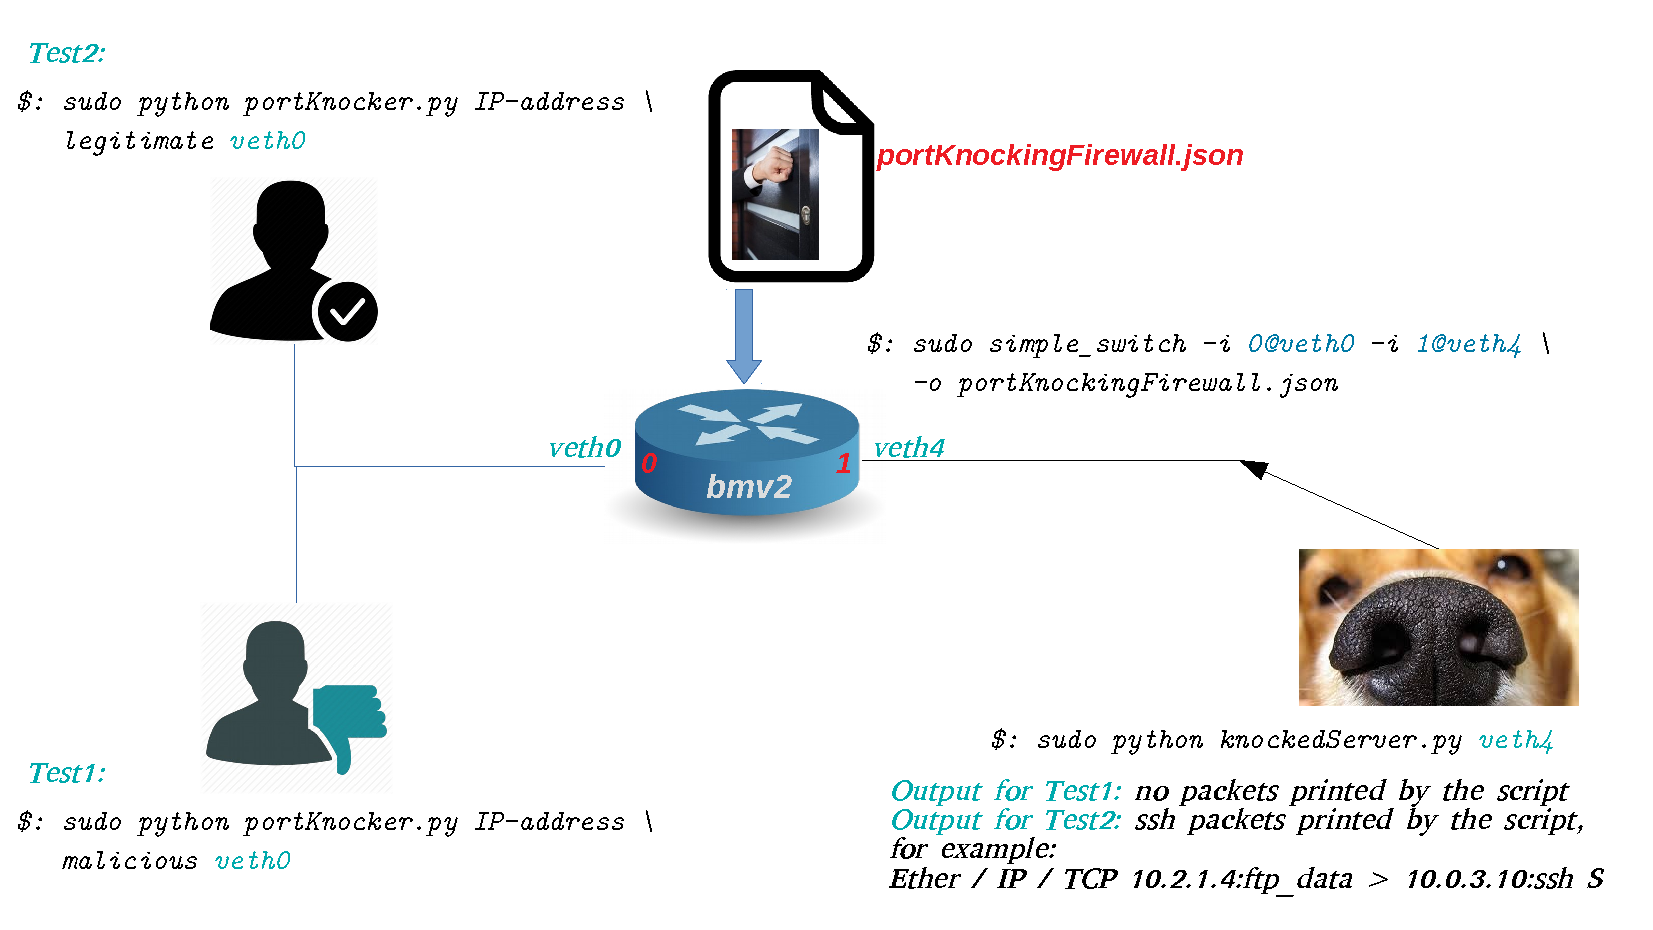
\includegraphics[width=1\textwidth]{./images/testPortKnockFw.pdf}
~\\
\subproblem{Submission} We expect you to deliver a P4 program (p4 source files and table entries) which we can load into the switch and test by using the same two python scripts provided to you.

\newpage

\problem{2: Network Sketches}{10}
A sketch is a data structure that stores summary information about network traffic captured through streaming, using a combination of hashing, counting and filtering techniques. Your task consists of implementing two sketching algorithms: Count-min and Bitmap.\\
The \textbf{Count-min Sketch} is a probabilistic data structure that serves as a frequency table of events in a stream of data. It uses hash functions to map events to frequencies, with a table for each function. For each event in a stream, various hash functions are calculated, and for each one, the respective table counters are incremented. The final value for a given event is a minimum among all tables.\\
The \textbf{Bitmap Sketch} counts the number of unique elements in a stream using an array of bits. Each stream event is hashed to a specific array position, where its value is changed from 0 to 1. The final sketch value is given by the sum of all the array values. For example, to count the number of unique sources accessing a web server via port 80, we can simply filter the traffic based on port 80 and then use a bitmap to count the number of unique source addresses.\\
~\\
\textbf{Implementation Guidelines}\\
Your \textbf{count-min sketch} implementation should contain three counters which identify flows based on the source and destination IP address. The hash input fields for each counter must be:
\begin{enumerate}
    \item cm\_hash\_0: hdr.ipv4.src\_addr, hdr.ipv4.dst\_addr, hdr.ipv4.version
    \item cm\_hash\_1: hdr.ipv4.src\_addr, hdr.ipv4.dst\_addr, hdr.ipv4.ihl
    \item cm\_hash\_2: hdr.ipv4.src\_addr, hdr.ipv4.dst\_addr   
\end{enumerate}

The final count-min values must be stored in a P4 register named cm\_register\_final and indexed by the hash cm\_hash\_2.\\

Your \textbf{bitmap sketch} implementation should store the number of unique destination IP addresses for each source IP address. The final sketch values must be stored in a P4 register named bm\_register\_final.\\

For the sake of this assignment, all registers used to store sketches values in your P4 programs must have a size of 131072 and the hash algorithms crc32 must be used to compute all the hashes.\\

The following steps illustrate a typical workflow to work on this task:
\begin{enumerate}
\item Unzip to a folder the p4\_sketches archive:\\
        \textit{\$: unzip problem2.zip} 
\item Edit the template of the main program:\\
        \textit{\$: vim p4\_sketches.p4}
\item Iteratively compile and fix your P4 code:\\
        \textit{\$: p4c-bm2-ss --arch v1model p4\_sketches.p4 -o p4\_sketches.json}
\item Create some veth interfaces and start the bmv2 switch:\\
        \textit{\$: sudo bash ./veth\_setup.sh}\\
        \textit{\$: sudo simple\_switch -i 0@Node1 \$FULL\_PATH\_TO\_YOUR/p4\_sketches.json}
\item Install the tcpreplay utility with the following:\\
        \textit{\$: sudo apt-get install tcpreplay}\\~\\
Test your program by opening two terminals and using the following commands:\\

- Send one of the provided pcap files on the /pcap/ folder to the switch with a packet replaying program, \textit{e.g.}, TcpReplay:\\

        \textit{\$: sudo tcpreplay -i Node1 -K -l 1 --pps=50 test\_cm.pcap}\\

- after replaying the pcap, read the sketches values from the switch through:\\

        \textit{\$: python p4\_sketches\_test.py cm \$FULL\_PATH\_TO\_YOUR/p4\_sketches.json}\\

as a result of the last command the sketch values are written into a txt file (either cm\_results.txt or bm\_results.txt according to the input different parameter, respectively 'cm' or 'bm', you specify).\\
- Compare the generated file (e.g., cm\_results.txt) against the correct sketch values provided to you (e.g., in cm\_final.txt).

\end{enumerate}

\subproblem{Submission} We expect you to deliver a P4 program (p4 source files and table entries, if any) which we can load into the switch to reply the same pcap files and obtain the same sketches values as you.

\newpage

\problem{3: Network Coding}{4}
Network coding is a network paradigm where intermediate nodes in the network can compute functions on the incoming packets and send new packets on their output links. With this simple shift in the networking paradigm, Network coding promises to offer benefits along several dimensions such as throughput, security and resilience to link failures and packet losses.\\
The  benefit of network coding are often illustrated with the classic “Butterfly network” example shown in the figure below where S  is  the source and all the links have the same capacity. The goal is to maximize the receiving rate at the two receivers R1 and R2  in a multicast session. Without network coding, the optimal throughput of 1.5 packets/channel use can be achieved, while, with  network  coding,  if peer X  is able  to code  its input messages a and b into a+b, an effective end-to-end throughput of 2 packets/channel use can be achieved instead.\\


\begin{center}

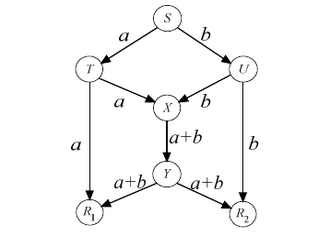
\includegraphics[scale=1]{./images/butterfly.png}

\end{center}

We ask you to emulate the butterfly topology in the picture in Mininet and deploy a P4 program on switch X that xor${s}$ packets' payloads.\\~\\~\\

\subproblem{Submission} This is an assignment for you to go wild with P4 and other tools you may have learned throughout this course (e.g., Mininet). Therefore, we are very open about the content of your submission. At the best, we would expect you to be able to implement this simple network coding function in P4, emulate the above topology with Mininet and showcase this function works at the end-hosts (for example, decoding by using a software library for network coding).



\end{document} 
